\subsection{El problema del punto único de falla}

Un servidor NFS centralizado simplifica la administracion del almacenamiento, pero tambien puede convertirse en un punto unico de falla. Si el servidor deja de responder, los clientes con montajes activos pueden bloquear operaciones de lectura o escritura, y las aplicaciones que dependen de esos archivos pueden quedar detenidas. En montajes \texttt{hard}, comportamiento recomendado para datos importantes, los procesos esperan hasta que el servidor vuelva a estar disponible.

Por esta razon, NFS en produccion requiere una estrategia de alta disponibilidad. No alcanza con tener un segundo servidor instalado: los clientes deben conservar una ruta estable hacia el servicio, el estado del protocolo debe recuperarse correctamente y los datos deben permanecer consistentes.

\subsection{Modelo activo/pasivo con IP virtual}

El diseño clasico de alta disponibilidad para NFS es un cluster activo/pasivo. Un nodo presta el servicio y posee una IP virtual. Los clientes montan los exports usando esa IP virtual, no la direccion fisica de un servidor concreto. Si el nodo activo falla, el cluster mueve la IP virtual al nodo pasivo, monta el almacenamiento correspondiente e inicia el servicio NFS.

Herramientas como Pacemaker y Corosync permiten coordinar recursos de cluster: IP virtual, montaje del volumen, servicio \texttt{nfsd} y orden de arranque. Este orden es importante: no tiene sentido publicar la IP antes de que el sistema de archivos este montado y el servicio listo para responder.

\begin{figure}[H]
    \centering
    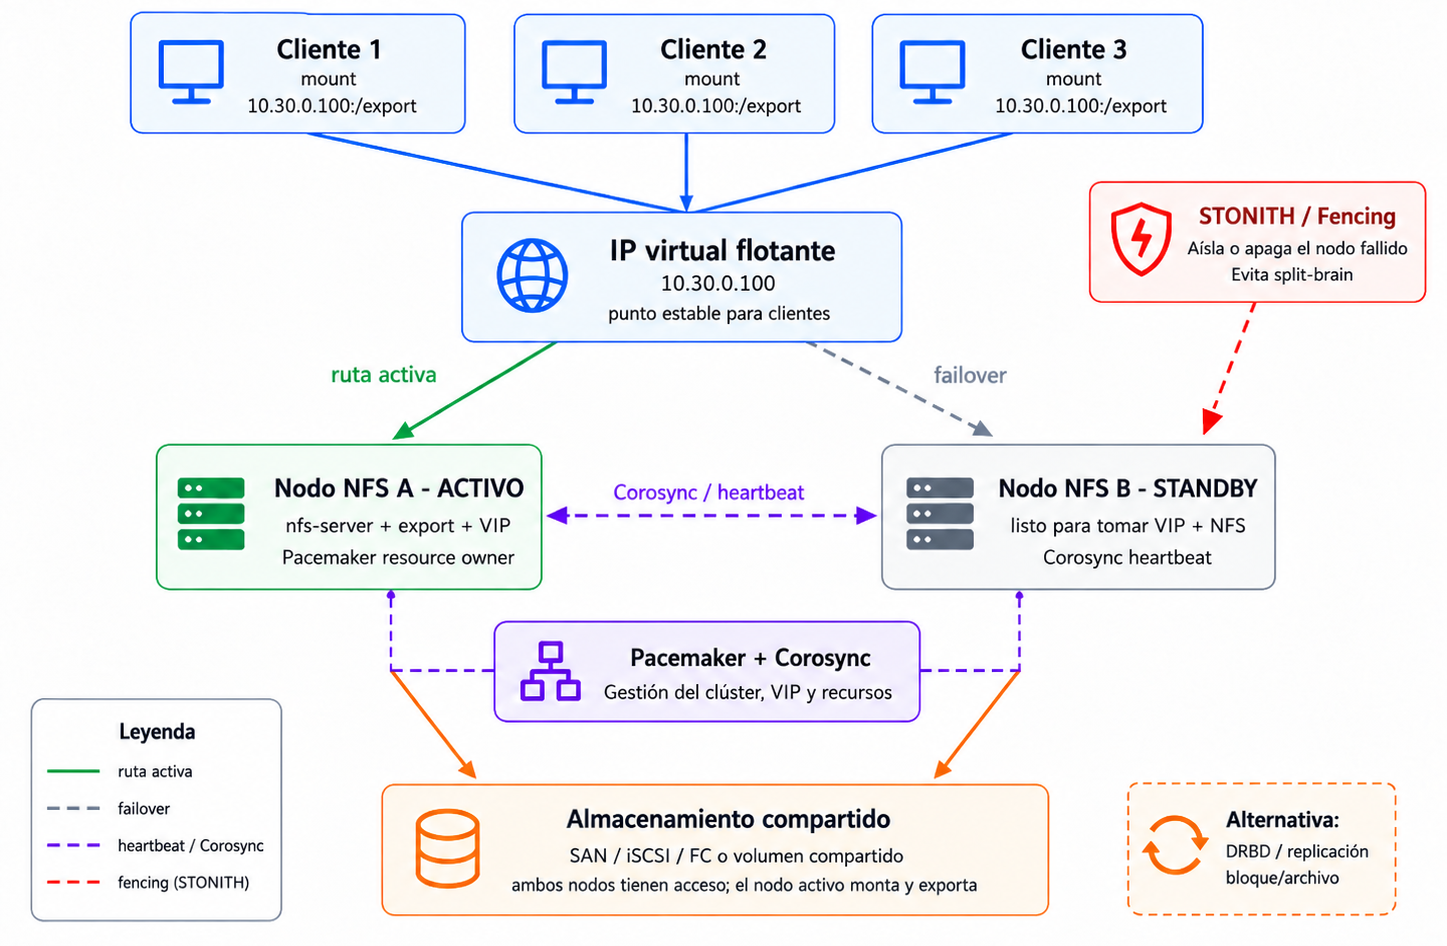
\includegraphics[width=0.95\textwidth]{img/nfs_05.png}
    \caption{Alta disponibilidad NFS activo/pasivo}
    \label{fig:nfs_ha}
\end{figure}

\subsection{Fencing, estado y consistencia}

El \textbf{fencing} es critico en cualquier cluster de almacenamiento. Si dos nodos creen simultaneamente que deben ser activos y escriben sobre los mismos datos, puede producirse corrupcion. Esta situacion se conoce como split-brain. Para evitarla, el cluster debe aislar o apagar de manera confiable al nodo dudoso antes de promover al nodo superviviente.

El cluster necesita que los datos esten disponibles para el nodo que toma el servicio. Esto puede resolverse mediante almacenamiento compartido, una cabina accesible por ambos servidores o replicacion entre nodos. En todos los casos, la prioridad es evitar escrituras simultaneas no coordinadas y asegurar que el nodo activo sea el unico que exporta el sistema de archivos.

Con NFSv4, el servidor mantiene estado: locks, opens, leases y sesiones. Durante un failover, el nuevo nodo debe poder recuperar ese estado o permitir que los clientes lo reclamen durante un periodo de gracia. Por eso, la alta disponibilidad de NFS no es solo mover una IP; tambien implica coordinar almacenamiento, servicio y estado del protocolo.

Alta disponibilidad y escalabilidad no son lo mismo. Un cluster activo/pasivo mejora la continuidad del servicio, pero no duplica el rendimiento porque solo un nodo atiende el trafico en condiciones normales. Para escalar capacidad se requieren otros enfoques, como NAS scale-out o pNFS, que deben evaluarse segun la carga y el presupuesto.
